\documentclass[aspectratio=32]{beamer}
\usepackage{hyperref}
\usepackage[utf8]{inputenc}
\usepackage{tikz}
\usepackage{graphicx}

\title{The Reality and Perception of Cybercrime in the European Union}
\author{Tristan Goodell}
\institute[]{Arkansas School for Mathematics, Sciences, and the Arts}
\date{14 October 2019}

\begin{document}
{
\usebackgroundtemplate{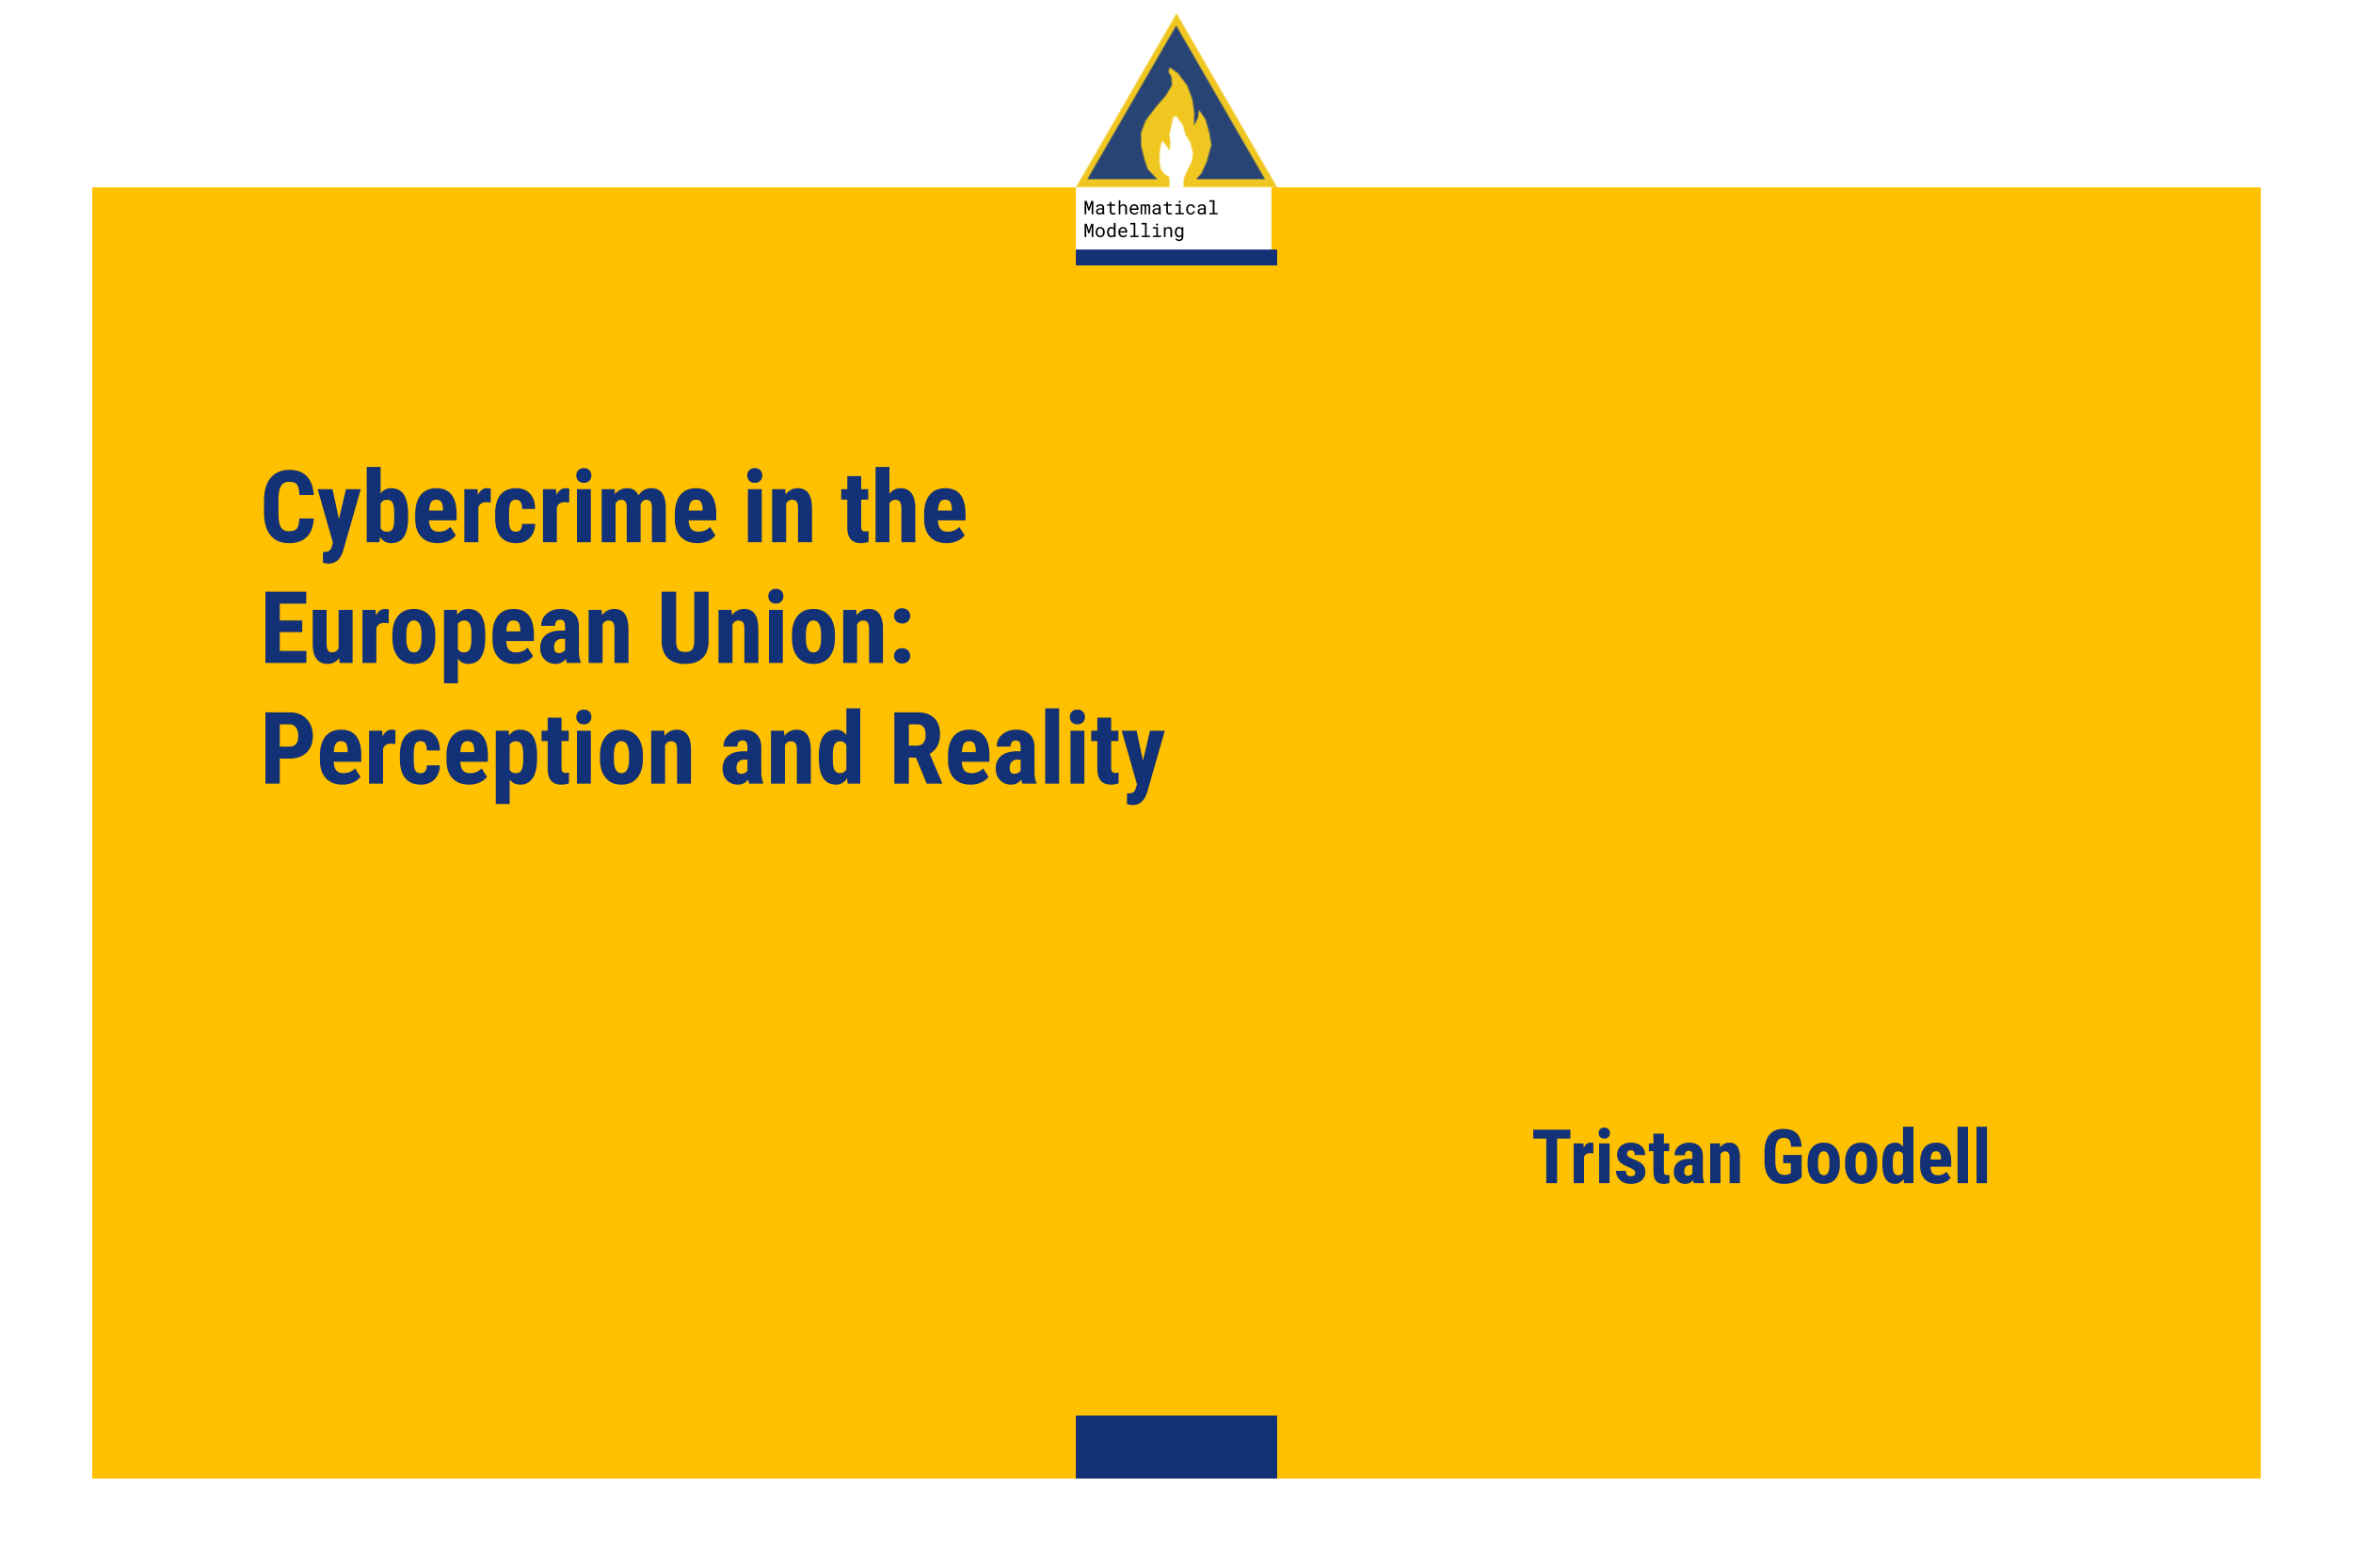
\includegraphics[width=\paperwidth]{title-slide.png}}
\begin{frame}{}

\end{frame}
}

\begin{frame}{Why Europe?}

\begin{itemize}
    \item Historically, the European Union (EU) has been incredibly transparent and liberal with its statistics and research with initiatives like the Eurobarometers--- public opinion surveys given by the European Commission starting in 1974. 
    \item Currently, the United States lacks a similar coordinated research effort. Consequently, the US lacks accessible data for cybercrime and cybersecurity in general.
    \item In the EU, Special Eurobarometers from 2012 to 2019 have been recording the perception of cybercrime in addition to other invaluable pieces of information, such as internet accessibility and use.
    \item This data will be combined with data concerning trends in cybercrime to construct the capstone project.
    \begin{figure}
        
\includegraphics[width=55pt]{eu.png}
    \end{figure}
\end{itemize}

\end{frame}

\begin{frame}{Rationale}
This project aims to:
    \begin{itemize}
        \item Analyze the correlation between perception of cybercrime and actual cybercrime.
        \item Display the relationship between internet access/use and various factors, such as country.
        \item Determine the effect EU legislation has had on the perception and reality of cybercrime.
        \item Establish a timeline consisting of all major data breaches, privacy scandals, EU Legislation, internet market penetration, perception of cybercrime from 2012 to 2018, and other statistics of note.
        \item Anything else that is deemed noteworthy and/or neccessary. 
    \end{itemize}
\end{frame}

\begin{frame}{Research Goals}
    \begin{itemize}
        \item The goal of this project is to determine if EU legislation, in addition to other EU funded endeavors, have an effect on the perception of cybercrime in the EU, actual cybercrime in the EU, and internet access for EU citizens. 
        \item Better understand the relationship between the perception and reality of cybercrime.
        \item Analyze trends in cybercrime in the EU. 
        \item Predict future trends, breaches, and legislative goals.
        \item Encourage the United States to collect data on cybercrime and make it publicly available so that future research can be done on cybercrime in the United States.
    \end{itemize}
\end{frame}

\begin{frame}{Procedures}

\begin{itemize}
    \item Phase I: Process the raw data in preparation for analysis.
    \item Phase II: Analyze the data using statistical and data science methods.
    \item Phase III: Construct models relevant to the Rationale and Research Goals.
    \item Phase IV: Write the paper in LaTeX. 
    \item Phase V: Present at Science Fair. 
    \begin{figure}
        
\includegraphics[width=70pt]{isef.png}
    \end{figure}
\end{itemize}

\end{frame}

\begin{frame}{Data}

\begin{itemize}
    \item 5 Eurobarometers
    \item 140 Factsheets
    \item 149 Spreadsheets of Field Data
    \item Have I Been Pwned's "Pwned Websites" List
    \item Numerous background research papers, such as IOCTA 2018.
    \begin{figure}
        
\includegraphics[width=100pt]{eu-commission.png}
        
\includegraphics[width=75pt]{europol.png}
    \end{figure}
\end{itemize}

\end{frame}



\end{document}
